The fixed search screened 137,430 states and directly checked 512 distinct disagreements. It found 223 cases meeting the complete action-margin and cross-refinement witness criterion.
A refinement-stable witness is candidate 48408, with $n=12$, $q=2$, $x=1$ and $p=(0.025081, 0.461728, 0.315619, 0.197572)$. It is reached by the separate public exploration process, not selected from policy evaluation.
The direct joint-belief backup selects ask deep (ID 2); weighted-Q selects abstain (ID 0); keeping the same joint-belief continuation but freezing model weights selects abstain (ID 0).
\begin{center}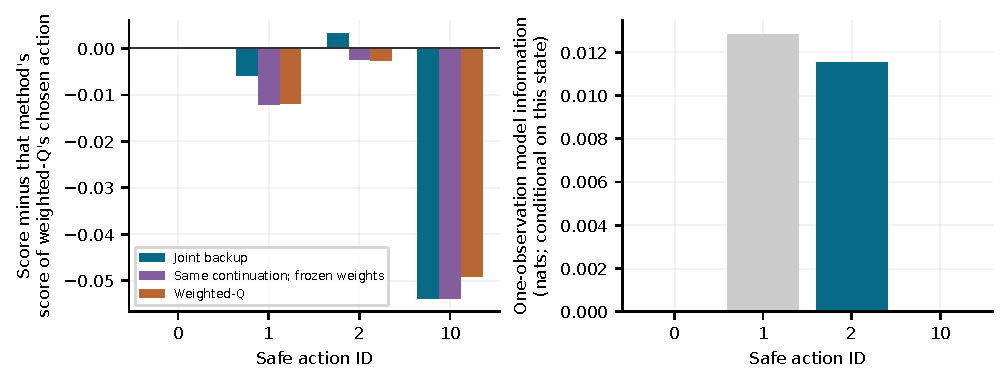
\includegraphics[width=\linewidth]{generated/action_explanation.pdf}\end{center}
{\small\textbf{Decision diagnostic.} Each score is centered on that same method's score of the weighted-Q action; absolute relaxed and feasible values are not subtracted. Positive information does not itself establish economic benefit.}
\begin{center}\small\begin{tabular}{lrr}\toprule
Quantity & Joint-belief choice & Weighted-Q choice\\\midrule
Immediate expected reward & +0.0460881 & +0.0520000\\
Model information (nats) & +0.0115330 & +0.0000000\\
Regime information conditional on model & +0.0214307 & +0.0000000\\
\bottomrule\end{tabular}\end{center}
